% !TeX program = xelatex
% ============================================================
% Modelo de Banco de Dados — RadarTorres
%
% Documento acadêmico individual (módulo do TCC), com no máximo
% 5 páginas, pensado para futuramente ser incorporado ao documento
% principal do TCC junto com os demais módulos (UML, Requisitos,
% Arquitetura, POO, Diagrama de Classes, Ferramentas).
%
% Estrutura e aparência visual (hierarquia de títulos, organização
% de figuras/tabelas, apresentação limpa) baseadas no template
% "UFMG Estruturas de Dados — Modelo geral de documentação para TP"
% (Overleaf: ufmg-estruturas-de-dados-modelo-geral-de-documentacao-para-tp).
% Não foram preservadas referências à UFMG/disciplina original —
% apenas a organização visual do modelo.
%
% Compile com XeLaTeX (usa a fonte Times New Roman do Windows
% diretamente, sem depender de pacotes extras do CTAN que não
% puderam ser baixados nesta instalação do MiKTeX — mesma
% abordagem já usada em Docs/Documentos_Entregaveis/TCC_Template_UCL.tex).
% ============================================================
\documentclass[11pt,a4paper]{article}

% ---------- Fonte: Times New Roman via XeLaTeX (sem babel/inputenc) ----------
\usepackage{fontspec}
\setmainfont{Times New Roman}

% ---------- Margens: 2,5 cm em todos os lados ----------
\usepackage[a4paper,margin=2.5cm]{geometry}

% ---------- Figuras e tabelas (diagramas ER reaproveitados de
% Modelo_Banco_de_Dados.md, nesta mesma pasta, como imagem — não TikZ) ----------
\usepackage{graphicx}
\usepackage{array}

% ---------- Nomes em português (sem depender do pacote "babel") ----------
\renewcommand{\figurename}{Figura}
\renewcommand{\tablename}{Tabela}

% ---------- Parágrafo: sem recuo, pequeno espaço entre parágrafos ----------
\setlength{\parindent}{0pt}
\setlength{\parskip}{4pt}

% ---------- Identificação (dados confirmados em Docs/Documentos_Entregaveis/TCC_Template_UCL.tex) ----------
\title{\vspace{-2em}
  {\normalsize Trabalho de Conclusão de Curso de Engenharia da Computação}\\[.4em]
  {\large\bfseries Protótipo para detecção, localização e seleção automática de ação por sensoriamento}\\[.2em]
  {\Large\bfseries Modelo de Banco de Dados}}
\author{
  \normalsize Gabriel Vasconcellos de Morais \quad--\quad Matheus Emanoel Gomes Souza\\[.3em]
  \small Orientador: Anker Douglas Loss\\
  \small Curso: Engenharia da Computação --- Faculdade do Centro Leste (UCL)
}
\date{}

\begin{document}
\maketitle
\vspace{-2em}

% ============================================================
% Conteúdo acadêmico puro do documento "Modelo de Banco de Dados".
% SEM \documentclass, \begin{document}/\end{document} nem título —
% pensado para ser reaproveitado via \input{} tanto no documento
% modular quanto, futuramente, no TCC principal.
% ============================================================

\section{Apresentação do Modelo de Dados}

O RadarTorres é um protótipo que detecta alvos por sensoriamento, seleciona automaticamente a
torre mais adequada e permite o acionamento manual ou automático de um indicador demonstrativo.
Para cumprir esse papel, o sistema precisa preservar, entre execuções, dados de naturezas
distintas: contas de usuário e seus perfis de acesso, o histórico de objetos detectados pelo
radar, a auditoria de toda ação de acionamento e de toda troca de modo de operação, e os
chamados de suporte abertos pelos operadores.

Além dos dados de auditoria, o sistema mantém preferências de interface por usuário (idioma,
tema, tela inicial), o layout personalizado dos painéis (posição, tamanho e visibilidade de cada
card), as zonas mortas configuradas por um administrador e as configurações de ambiente do
Arduino (porta serial, placa, sketch). Cada grupo tem finalidade e ciclo de vida próprios, mas
todos precisam sobreviver ao fechamento da aplicação.

Por não depender de um servidor de banco de dados, o protótipo prioriza simplicidade de
instalação e execução local/offline — coerente com o estágio atual do projeto (protótipo
acadêmico, uso demonstrativo). As seções seguintes descrevem a tecnologia de persistência
empregada, suas vantagens e limitações, as principais entidades identificadas no código e o
modelo proposto para uma futura migração relacional.

\section{Tecnologia e Implementação}

O protótipo atual \textbf{não utiliza um Sistema Gerenciador de Banco de Dados relacional}. A
persistência é realizada localmente por meio de arquivos CSV e JSON, sem servidor e sem
instalação adicional — portanto não há uma \textit{versão de SGBD} a declarar.

Seis entidades usam arquivos \textbf{CSV}, um por tabela, em
\texttt{\%AppData\%}\allowbreak\texttt{\textbackslash RadarTorres}\allowbreak\texttt{\textbackslash
Data\textbackslash} (pasta do usuário do Windows, sem privilégio de administrador) — ver a
coluna "Persistência" da Tabela~\ref{tab:entidades}. Cada arquivo é criado com cabeçalho na
primeira execução por \texttt{CsvTableStore<T>}; não há \textit{migration} tradicional — o
próprio código (modelo + mapeamento de colunas) define o schema.

Outras três entidades usam arquivos \textbf{JSON} individuais em
\texttt{\%LocalAppData\%}\allowbreak\texttt{\textbackslash RadarTorres\textbackslash}: um único
arquivo por instalação para zonas mortas e para configurações do Arduino, e um arquivo por tela e
por usuário para o layout dos painéis (nome com o padrão
\texttt{dashboard-}\allowbreak\texttt{layout-\{tela\}-\{usuário\}.json}). Cada entidade é
acessada exclusivamente por uma interface de repositório dedicada (ex.:
\texttt{IUsuario}\allowbreak\texttt{Repository}, \texttt{IDeadZone}\allowbreak\texttt{Repository}),
isolando ViewModels e Services do formato de armazenamento.

\textbf{Implementação futura proposta:} existe um plano documentado de migração para um banco
relacional (SQLite ou Entity Framework Core), trocando apenas a implementação de cada
repositório sem alterar ViewModels/Services. Essa tecnologia \emph{ainda não foi implementada} —
não há arquivo de banco, tabela SQL ou \textit{migration} no repositório hoje.

\section{Vantagens e Limitações da Solução Atual}

\begin{table}[htbp]
  \centering
  \caption{Vantagens e limitações da persistência atual (CSV/JSON)}
  \label{tab:vantagens}
  \small
  \renewcommand{\arraystretch}{1.25}
  \begin{tabular}{p{6.6cm}p{6.6cm}}
    \hline
    \textbf{Vantagens} & \textbf{Limitações} \\
    \hline
    Simplicidade de instalação, sem servidor & Sem integridade referencial imposta pelo
    armazenamento \\
    Funcionamento local/offline & Consultas limitadas (sem SQL; filtragem em memória) \\
    Baixo acoplamento via interfaces de repositório & Tende a não escalar bem para grande
    volume de dados \\
    Fácil distribuição (basta copiar a pasta de dados) & Sem controle de concorrência/transações
    reais \\
    Adequado ao estágio atual de protótipo & Relacionamentos garantidos só pelo código da
    aplicação \\
    \hline
  \end{tabular}
\end{table}

Essas limitações não indicam uma decisão equivocada: CSV/JSON atendem plenamente ao escopo de um
protótipo de uso demonstrativo. A Seção~\ref{sec:proposto} apresenta o modelo pensado para quando
a evolução do projeto exigir um SGBD relacional.

\section{Principais Dados do Sistema}

\begin{table}[htbp]
  \centering
  \caption{Entidades persistidas identificadas no código-fonte}
  \label{tab:entidades}
  \small
  \renewcommand{\arraystretch}{1.2}
  \begin{tabular}{p{3.1cm}p{5.8cm}p{4.1cm}}
    \hline
    \textbf{Entidade} & \textbf{Finalidade} & \textbf{Persistência} \\
    \hline
    Usuario & Conta de acesso, perfil e autenticação & CSV\newline\scriptsize\texttt{usuarios.csv} \\
    PreferenciasUsuario & Preferências de interface por usuário &
    CSV\newline\scriptsize\texttt{preferencias\_}\allowbreak\texttt{usuario.csv} \\
    ObjetoDetectado & Histórico de detecções do radar &
    CSV\newline\scriptsize\texttt{objetos\_}\allowbreak\texttt{detectados.csv} \\
    AcaoRealizada & Auditoria de acionamentos (só inserção) &
    CSV\newline\scriptsize\texttt{acoes\_}\allowbreak\texttt{realizadas.csv} \\
    AlteracaoModo & Auditoria de troca de modo de operação &
    CSV\newline\scriptsize\texttt{alteracoes\_}\allowbreak\texttt{modo.csv} \\
    ChamadoAjuda & Chamados de suporte dos usuários &
    CSV\newline\scriptsize\texttt{chamados\_}\allowbreak\texttt{ajuda.csv} \\
    DeadZone & Áreas onde alvos são ignorados pelo sistema &
    JSON\newline\scriptsize\texttt{dead-zones.json} \\
    Dashboard\allowbreak CardLayout & Layout dos cards do painel, por tela/usuário &
    JSON\newline\scriptsize\texttt{dashboard-}\allowbreak\texttt{layout-*.json} \\
    ArduinoSettings & Configurações de ambiente do Arduino &
    JSON\newline\scriptsize\texttt{arduino-}\allowbreak\texttt{settings.json} \\
    \hline
  \end{tabular}
\end{table}

\section{Modelo e Relacionamentos}
\label{sec:modelo}

A Figura~\ref{fig:atual} reproduz o Diagrama Entidade-Relacionamento já levantado para as seis
entidades em CSV (arquivo \texttt{Modelo\_Banco\_de\_Dados.md}, nesta mesma pasta).

\texttt{Usuario} se relaciona 1:1 com \texttt{PreferenciasUsuario} (chave \texttt{UsuarioId},
igual a \texttt{Usuario.Id}) e 1:N com \texttt{AcaoRealizada} e \texttt{AlteracaoModo} — nesses
dois últimos casos por \textbf{Login} (texto), sem chave estrangeira real — e com
\texttt{ChamadoAjuda}, por \texttt{Id} numérico. \texttt{ObjetoDetectado} \textbf{não possui
nenhum vínculo persistido} com \texttt{AcaoRealizada}, \texttt{Usuario} ou qualquer outra
entidade — são registros independentes, como o próprio diagrama mostra (sem linha de
relacionamento).

\begin{figure}[htbp]
  \centering
  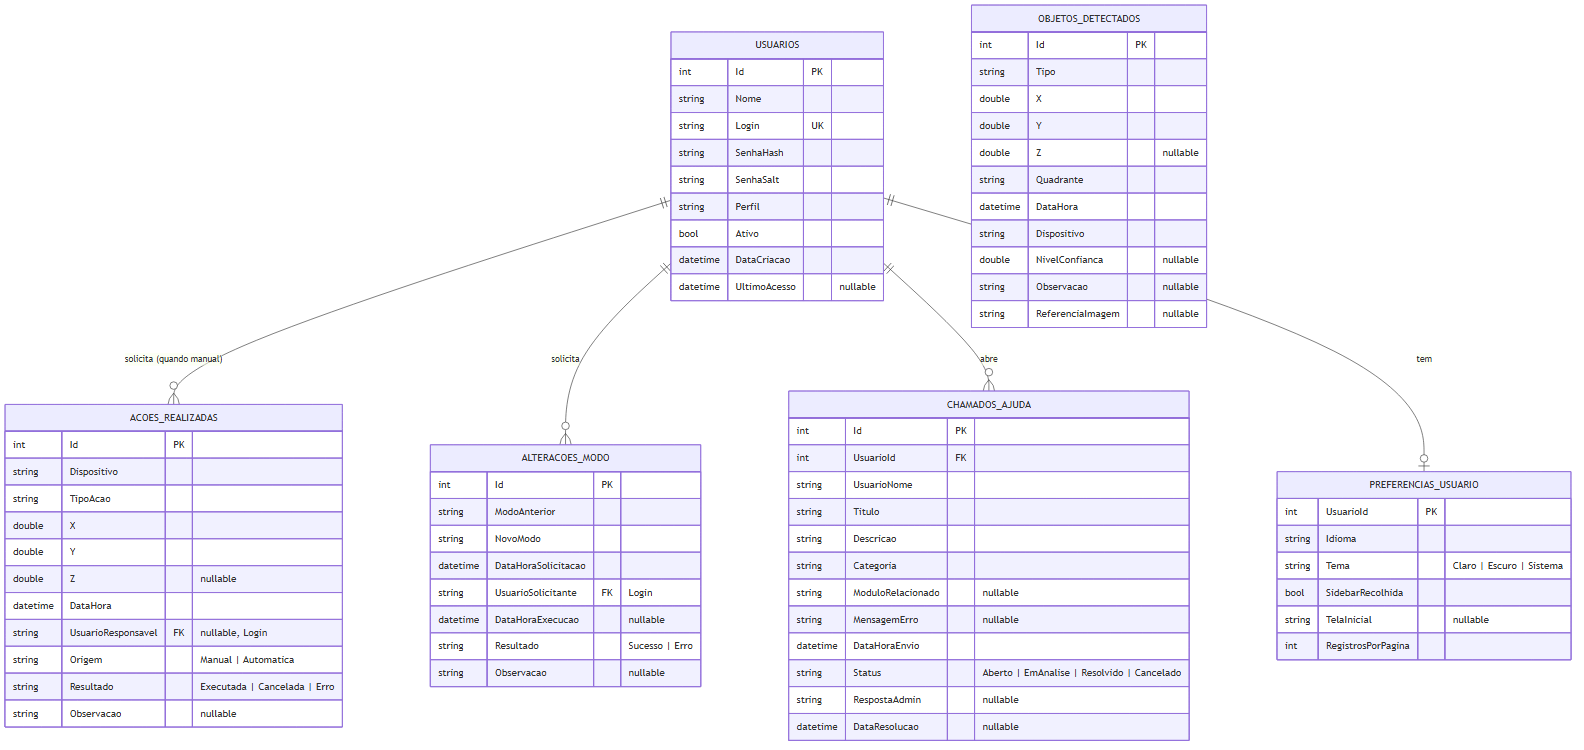
\includegraphics[width=\textwidth]{figuras/DER_Atual.png}
  \caption{Modelo de dados atual (persistência em CSV) — diagrama entidade-relacionamento já
  levantado a partir do código-fonte do projeto.}
  \label{fig:atual}
\end{figure}

{\sloppy
Três entidades adicionais usam arquivos JSON e não aparecem no diagrama acima, por não
fazerem parte do levantamento original de CSV (ver Tabela~\ref{tab:entidades}):
\texttt{DeadZone}, \texttt{Dash\-board\-Card\-Layout} e \texttt{ArduinoSettings}. Nenhuma delas tem
relacionamento persistido com \texttt{Usuario} ou entre si: \texttt{DeadZone} e
\texttt{ArduinoSettings} são configurações únicas por instalação, e \texttt{Dash\-board\-Card\-Layout}
se associa a um usuário apenas pelo \emph{nome do arquivo} (\texttt{tela-idUsuario}) — uma
convenção de nomenclatura, não uma chave estrangeira — por isso não são representadas em um
diagrama ER à parte.\par}

\section{Modelo Relacional Proposto}
\label{sec:proposto}

\textbf{Esta seção descreve uma proposta de migração futura, não o banco atual} — nenhuma dessas
tabelas, chaves ou \textit{migrations} existe hoje no repositório. A estrutura de dados seria a
mesma da Figura~\ref{fig:atual}, mas as referências textuais por \texttt{Login} passariam a ser
chaves estrangeiras íntegras por \texttt{Id} numérico, com integridade garantida pelo próprio
SGBD (Figura~\ref{fig:proposto}). \texttt{ObjetosDetectados} permanece sem chave estrangeira, pelo
mesmo motivo já explicado na Seção~\ref{sec:modelo}.

\begin{figure}[htbp]
  \centering
  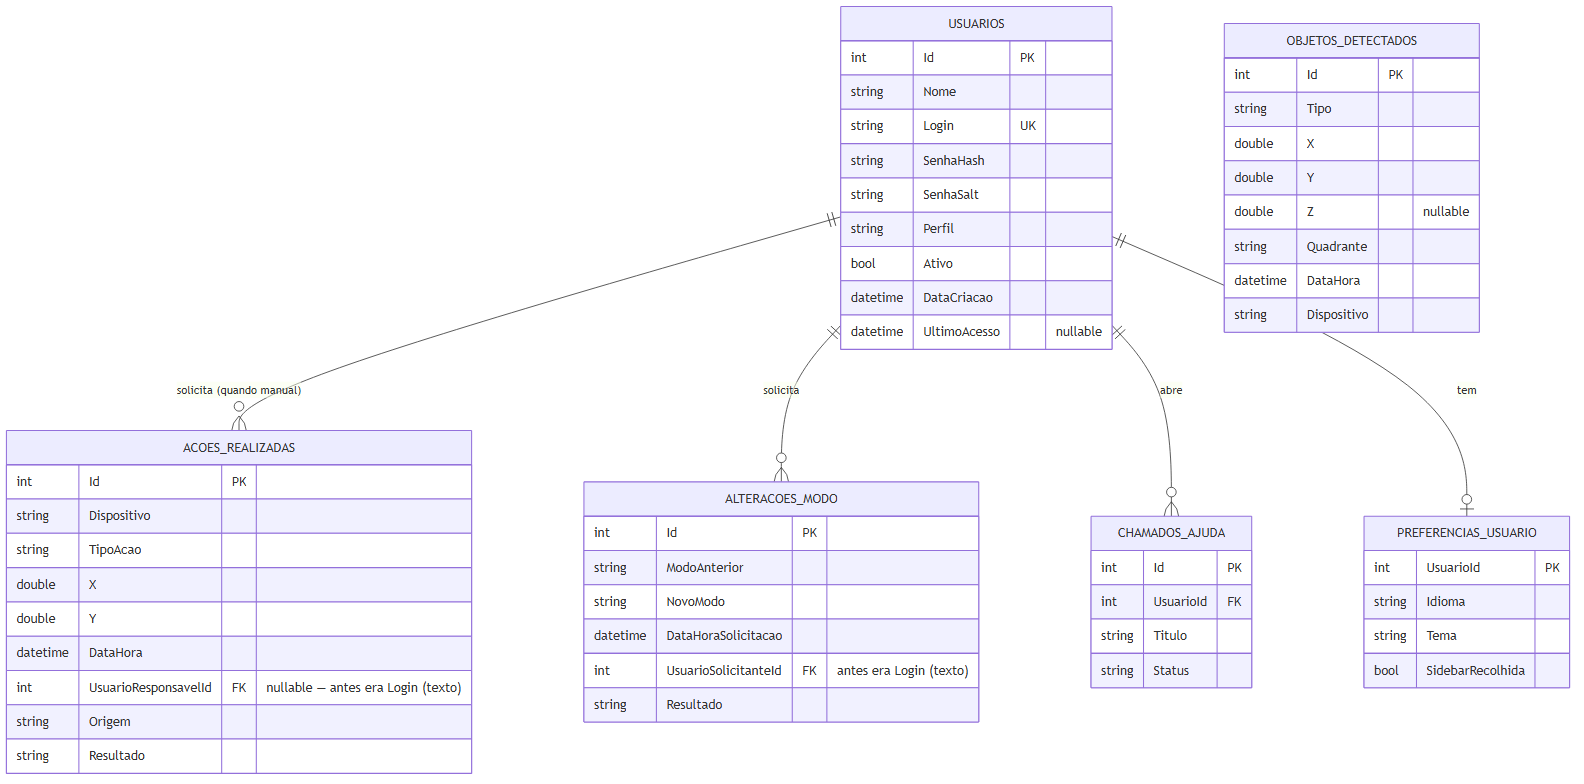
\includegraphics[width=\textwidth]{figuras/DER_Proposto.png}
  \caption{Modelo relacional proposto para a migração futura de persistência (CSV/JSON
  $\rightarrow$ SQL) — mesmo levantamento já documentado em
  \texttt{Modelo\_Banco\_de\_Dados.md} (nesta mesma pasta).}
  \label{fig:proposto}
\end{figure}

\section{Conclusão}

A persistência atual, baseada em arquivos CSV e JSON, atende plenamente ao estágio de protótipo
do RadarTorres, mantendo a instalação simples e o funcionamento totalmente local. O uso de uma
interface de repositório dedicada para cada entidade mantém a camada de dados desacoplada das
demais camadas da aplicação, o que viabiliza uma futura migração para um banco relacional de
forma incremental, sem exigir mudanças em ViewModels ou Services. O modelo atual já preserva as
informações necessárias de operação, auditoria e configuração exigidas pelo sistema.

\section*{REFERÊNCIAS}
\small
\raggedright
[REFERÊNCIA BIBLIOGRÁFICA A INSERIR]


\end{document}
